\begin{frame}{QR Decomposition}
    \begin{itemize}
        \item A rectangular matrix $A\in \mathbb{R}^{m \times n}$ can be decomposed into an orthogonal matrix $Q$ and an upper triangular matrix $R$ such that:
        \begin{align*}
            A = QR
        \end{align*}
    where $Q\in \mathbb{R}^{m \times m}$ is orthogonal ($Q^T Q = I$) and $R\in \mathbb{R}^{m \times n}$ is upper triangular.
    \end{itemize}
\end{frame}

\begin{frame}
 \begin{figure}
        \begin{center}
        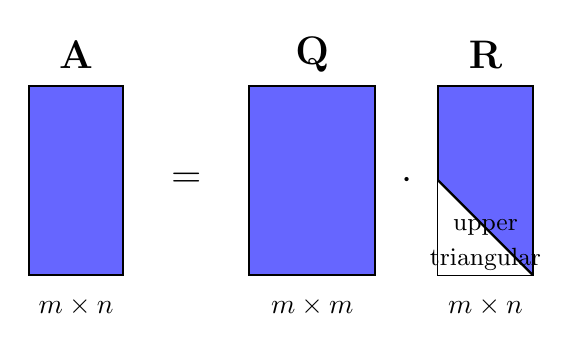
\begin{tikzpicture}[scale=0.8]
            % Matrix A (m x n)
            \fill[blue!60] (0,0) rectangle (1.5,3);
            \draw[thick] (0,0) rectangle (1.5,3);
            \node[font=\Large\bfseries] at (0.75,3.5) {A};
            \node at (0.75,-0.5) {$m \times n$};
            
            % Equals sign
            \node[font=\Large] at (2.5,1.5) {=};
            
            % Matrix Q (m x m)
            \fill[blue!60] (3.5,0) rectangle (5.5,3);
            \draw[thick] (3.5,0) rectangle (5.5,3);
            \node[font=\Large\bfseries] at (4.5,3.5) {Q};
            \node at (4.5,-0.5) {$m \times m$};
            
            % Multiplication dot
            \node[font=\Large] at (6,1.5) {$\cdot$};
            
            % Matrix R (m x n) - upper triangular
            \fill[blue!60] (6.5,0) rectangle (8,3);
            \draw[thick] (6.5,0) rectangle (8,3);
            
            % Draw upper triangular pattern
            \fill[white] (6.5,0) -- (8,0) -- (6.5,1.5) -- cycle;
            \draw[thick] (6.5,1.5) -- (8,0);
            
            \node[font=\Large\bfseries] at (7.25,3.5) {R};
            \node at (7.25,-0.5) {$m \times n$};
            \node[font=\small] at (7.25,0.75) {upper};
            \node[font=\small] at (7.25,0.25) {triangular};
        \end{tikzpicture}
        \end{center}
        \caption{QR Decomposition: $A = QR$ where $Q$ is orthogonal and $R$ is upper triangular}
    \end{figure}
\end{frame}

\begin{frame}
    \begin{itemize}
        \item Example: For a matrix $A$:
        {\small
        \begin{align*}
            A = \begin{bmatrix}
                1 & 2 & 3 \\    
                4 & 5 & 6 \\
                7 & 8 & 9
            \end{bmatrix}
        \end{align*}
        The QR decomposition yields:
        \begin{align*}
            Q = \begin{bmatrix}
                -0.123 & -0.904 & 0.408 \\
                -0.492 & -0.301 & -0.816 \\
                -0.861 & 0.301 & 0.408
            \end{bmatrix}, \quad
            R = \begin{bmatrix}
                -8.124 & -9.904 & -11.684 \\
                0 & 0.904 & 1.632 \\
                0 & 0 & 0
            \end{bmatrix}
        \end{align*}
        where $Q^T Q = I$ and $R$ is upper triangular.
        }
    \end{itemize}
\end{frame}

\begin{frame}
    \begin{block}{\textbf{QR Decomposition Theorem:}} For any matrix $A \in \mathbb{R}^{m \times n}$, there exists a matrix $Q \in \mathbb{R}^{m \times m}$ and a matrix $R \in \mathbb{R}^{m \times n}$ such that:
        \begin{align*}
            A = QR
        \end{align*}
        where $Q^T Q =QQ^T=I_m$ and $R$ is upper triangular.
    \end{block}
\end{frame}

\begin{frame}
    \begin{itemize}
        \item \textbf{QR Algorithm:}
        \begin{enumerate}
            \item Initialize: $A^{(0)} = A$
            \item For $k = 0, 1, 2, \ldots$ until convergence:
            \begin{itemize}
                \item Compute QR decomposition: $A^{(k)} = Q^{(k)} R^{(k)}$
                \item Update: $A^{(k+1)} = R^{(k)} Q^{(k)}$
            \end{itemize}
            \item As $k \to \infty$, $A^{(k)}$ converges to an upper triangular matrix
            \item The diagonal elements of the limit matrix are the eigenvalues of $A$
        \end{enumerate}
        \item \textbf{Key insight:} Each iteration preserves eigenvalues since $A^{(k+1)}$ is similar to $A^{(k)}$
    \end{itemize}
\end{frame}

\begin{frame}
    \begin{itemize}
        \item How do we compute $Q$ and $R$?
        \item The Gram-Schmidt process is a common method:
        \begin{itemize}
            \item Start with the columns of $A$ as vectors.
            \item Orthogonalize them to form $Q$.
            \item Normalize to ensure orthonormality.
            \item Form $R$ from the coefficients of the linear combinations.   
    \end{itemize}
\end{itemize}
\end{frame}
\begin{frame}
    
\end{frame}